% Lines starting with a percent sign (%) are comments. LaTeX will 
% not process those lines. Similarly, everything after a percent 
% sign in a line is considered a comment. To produce a percent sign
% in the output, write \% (backslash followed by the percent sign). 
% ==================================================================
% Usage instructions:
% ------------------------------------------------------------------
% The file is heavily commented so that you know what the various
% commands do. Feel free to remove any comments you don't need from
% your own copy. When redistributing the example thesis file, please
% retain all the comments for the benefit of other thesis writers! 
% ==================================================================
% Compilation instructions: 
% ------------------------------------------------------------------
% Use pdflatex to compile! Input images are expected as PDF files.
% Example compilation:
% ------------------------------------------------------------------
% > pdflatex thesis-example.tex
% > bibtex thesis-example
% > pdflatex thesis-example.tex
% > pdflatex thesis-example.tex
% ------------------------------------------------------------------
% You need to run pdflatex multiple times so that all the cross-references
% are fixed. pdflatex will tell you if you need to re-run it (a warning
% will be issued)  
% ------------------------------------------------------------------
% Compilation has been tested to work in ukk.cs.hut.fi and kosh.hut.fi
% - if you have problems of missing .sty -files, then the local LaTeX
% environment does not have all the required packages installed.
% For example, when compiling in vipunen.hut.fi, you get an error that
% tikz.sty is missing - in this case you must either compile somewhere
% else, or you cannot use TikZ graphics in your thesis and must therefore
% remove or comment out the tikz package and all the tikz definitions. 
% ------------------------------------------------------------------

% General information
% ==================================================================
% Package documentation:
% 
% The comments often refer to package documentation. (Almost) all LaTeX
% packages have documentation accompanying them, so you can read the
% package documentation for further information. When a package 'xxx' is
% installed to your local LaTeX environment (the document compiles
% when you have \usepackage{xxx} and LaTeX does not complain), you can 
% find the documentation somewhere in the local LaTeX texmf directory
% hierarchy. In ukk.cs.hut.fi, this is /usr/texlive/2008/texmf-dist,
% and the documentation for the titlesec package (for example) can be 
% found at /usr/texlive/2008/texmf-dist/doc/latex/titlesec/titlesec.pdf.
% Most often the documentation is located as a PDF file in 
% /usr/texlive/2008/texmf-dist/doc/latex/xxx, where xxx is the package name; 
% however, documentation for TikZ is in
% /usr/texlive/2008/texmf-dist/doc/latex/generic/pgf/pgfmanual.pdf
% (this is because TikZ is a front-end for PGF, which is meant to be a 
% generic portable graphics format for LaTeX).
% You can try to look for the package manual using the ``find'' shell
% command in Linux machines; the find databases are up-to-date at least
% in ukk.cs.hut.fi. Just type ``find xxx'', where xxx is the package
% name, and you should find a documentation file.
% Note that in some packages, the documentation is in the DVI file
% format. In this case, you can copy the DVI file to your home directory,
% and convert it to PDF with the dvipdfm command (or you can read the
% DVI file directly with a DVI viewer).
% 
% If you can't find the documentation for a package, just try Googling
% for ``latex packagename''; most often you can get a direct link to the
% package manual in PDF format.
% ------------------------------------------------------------------


% Document class for the thesis is report
% ------------------------------------------------------------------
% You can change this but do so at your own risk - it may break other things.
% Note that the option pdftext is used for pdflatex; there is no
% pdflatex option. 
% ------------------------------------------------------------------
\documentclass[12pt,a4paper,oneside,pdftex]{report}

% The input files (tex files) are encoded with the latin-1 encoding 
% (ISO-8859-1 works). Change the latin1-option if you use UTF8 
% (at some point LaTeX did not work with UTF8, but I'm not sure
% what the current situation is) 
\usepackage[latin1]{inputenc}
% OT1 font encoding seems to work better than T1. Check the rendered
% PDF file to see if the fonts are encoded properly as vectors (instead
% of rendered bitmaps). You can do this by zooming very close to any letter 
% - if the letter is shown pixelated, you should change this setting 
% (try commenting out the entire line, for example).  
\usepackage[OT1]{fontenc}
% The babel package provides hyphenating instructions for LaTeX. Give
% the languages you wish to use in your thesis as options to the babel
% package (as shown below). You can remove any language you are not
% going to use.
% Examples of valid language codes: english (or USenglish), british, 
% finnish, swedish; and so on.
\usepackage[finnish,swedish,english]{babel}


% Font selection
% ------------------------------------------------------------------
% The default LaTeX font is a very good font for rendering your 
% thesis. It is a very professional font, which will always be 
% accepted. 
% If you, however, wish to spicen up your thesis, you can try out
% these font variants by uncommenting one of the following lines
% (or by finding another font package). The fonts shown here are 
% all fonts that you could use in your thesis (not too silly). 
% Changing the font causes the layouts to shift a bit; you many
% need to manually adjust some layouts. Check the warning messages
% LaTeX gives you.
% ------------------------------------------------------------------
% To find another font, check out the font catalogue from
% http://www.tug.dk/FontCatalogue/mathfonts.html
% This link points to the list of fonts that support maths, but
% that's a fairly important point for master's theses.
% ------------------------------------------------------------------
% <rant>
% Remember, there is no excuse to use Comic Sans, ever, in any
% situation! (Well, maybe in speech bubbles in comics, but there 
% are better options for those too)
% </rant>

% \usepackage{palatino}
% \usepackage{tgpagella}



% Optional packages
% ------------------------------------------------------------------
% Select those packages that you need for your thesis. You may delete
% or comment the rest.

% Natbib allows you to select the format of the bibliography references.
% The first example uses numbered citations: 
\usepackage[square,sort&compress,numbers]{natbib}
% The second example uses author-year citations.
% If you use author-year citations, change the bibliography style (below); 
% acm style does not work with author-year citations.
% Also, you should use \citet (cite in text) when you wish to refer
% to the author directly (\citet{blaablaa} said blaa blaa), and 
% \citep when you wish to refer similarly than with numbered citations
% (It has been said that blaa blaa~\citep{blaablaa}).
% \usepackage[square]{natbib}

% The alltt package provides an all-teletype environment that acts
% like verbatim but you can use LaTeX commands in it. Uncomment if 
% you want to use this environment. 
% \usepackage{alltt}

% The eurosym package provides a euro symbol. Use with \euro{}
\usepackage{eurosym} 

% Verbatim provides a standard teletype environment that renderes
% the text exactly as written in the tex file. Useful for code
% snippets (although you can also use the listings package to get
% automatic code formatting). 
\usepackage{verbatim}

% The listing package provides automatic code formatting utilities
% so that you can copy-paste code examples and have them rendered
% nicely. See the package documentation for details.
% \usepackage{listings}

% The fancuvrb package provides fancier verbatim environments 
% (you can, for example, put borders around the verbatim text area
% and so on). See package for details.
% \usepackage{fancyvrb}

% Supertabular provides a tabular environment that can span multiple 
% pages. 
%\usepackage{supertabular}
% Longtable provides a tabular environment that can span multiple 
% pages. This is used in the example acronyms file. 
\usepackage{longtable}

% The fancyhdr package allows you to set your the page headers 
% manually, and allows you to add separator lines and so on. 
% Check the package documentation. 
% \usepackage{fancyhdr}

% Subfigure package allows you to use subfigures (i.e. many subfigures
% within one figure environment). These can have different labels and
% they are numbered automatically. Check the package documentation. 
\usepackage{subfigure}

% The titlesec package can be used to alter the look of the titles 
% of sections, chapters, and so on. This example uses the ``medium'' 
% package option which sets the titles to a medium size, making them
% a bit smaller than what is the default. You can fine-tune the 
% title fonts and sizes by using the package options. See the package
% documentation.
\usepackage[medium]{titlesec}

% The TikZ package allows you to create professional technical figures.
% The learning curve is quite steep, but it is definitely worth it if 
% you wish to have really good-looking technical figures. 
\usepackage{tikz}
% You also need to specify which TikZ libraries you use
\usetikzlibrary{positioning}
\usetikzlibrary{calc}
\usetikzlibrary{arrows}
\usetikzlibrary{decorations.pathmorphing,decorations.markings}
\usetikzlibrary{shapes}
\usetikzlibrary{patterns}


% The aalto-thesis package provides typesetting instructions for the
% standard master's thesis parts (abstracts, front page, and so on)
% Load this package second-to-last, just before the hyperref package.
% Options that you can use: 
%   mydraft - renders the thesis in draft mode. 
%             Do not use for the final version. 
%   doublenumbering - [optional] number the first pages of the thesis
%                     with roman numerals (i, ii, iii, ...); and start
%                     arabic numbering (1, 2, 3, ...) only on the 
%                     first page of the first chapter
%   twoinstructors  - changes the title of instructors to plural form
%   twosupervisors  - changes the title of supervisors to plural form
\usepackage[mydraft]{aalto-thesis}
%\usepackage[mydraft,doublenumbering]{aalto-thesis}
%\usepackage{aalto-thesis}



\usepackage{mathtools}

\usepackage{graphicx}
\usepackage{wrapfig}



% Hyperref
% ------------------------------------------------------------------
% Hyperref creates links from URLs, for references, and creates a
% TOC in the PDF file.
% This package must be the last one you include, because it has
% compatibility issues with many other packages and it fixes
% those issues when it is loaded.   
\RequirePackage[pdftex]{hyperref}
% Setup hyperref so that links are clickable but do not look 
% different
\hypersetup{colorlinks=false,raiselinks=false,breaklinks=true}
\hypersetup{pdfborder={0 0 0}}
\hypersetup{bookmarksnumbered=true}
% The following line suggests the PDF reader that it should show the 
% first level of bookmarks opened in the hierarchical bookmark view. 
\hypersetup{bookmarksopen=true,bookmarksopenlevel=1}
% Hyperref can also set up the PDF metadata fields. These are
% set a bit later on, after the thesis setup.   


% Thesis setup
% ==================================================================
% Change these to fit your own thesis.
% \COMMAND always refers to the English version;
% \FCOMMAND refers to the Finnish version; and
% \SCOMMAND refers to the Swedish version.
% You may comment/remove those language variants that you do not use
% (but then you must not include the abstracts for that language)
% ------------------------------------------------------------------
% If you do not find the command for a text that is shown in the cover page or
% in the abstract texts, check the aalto-thesis.sty file and locate the text
% from there. 
% All the texts are configured in language-specific blocks (lots of commands
% that look like this: \renewcommand{\ATCITY}{Espoo}.
% You can just fix the texts there. Just remember to check all the language
% variants you use (they are all there in the same place). 
% ------------------------------------------------------------------
\newcommand{\TITLE}{Optimising and automating work planning by approximating
the vehicle routing problem} 
\newcommand{\FTITLE}{Ty�nsuunnittelun optimointi ja automatisointi k�ytt�en
heuristisia menetelmi� ajoneuvojen reititysongelmaan}
\newcommand{\STITLE}{Den stora stygga vargen}
\newcommand{\SUBTITLE}{}
\newcommand{\FSUBTITLE}{}
\newcommand{\SSUBTITLE}{}
\newcommand{\DATE}{June 18, 2011}
\newcommand{\FDATE}{18. kes�kuuta 2011}
\newcommand{\SDATE}{Den 18 Juni 2011}

% Supervisors and instructors
% ------------------------------------------------------------------
% If you have two supervisors, write both names here, separate them with a 
% double-backslash (see below for an example)
% Also remember to add the package option ``twosupervisors'' or
% ``twoinstructors'' to the aalto-thesis package so that the titles are in
% plural.
% Example of one supervisor:
%\newcommand{\SUPERVISOR}{Professor Antti Yl�-J��ski}
%\newcommand{\FSUPERVISOR}{Professori Antti Yl�-J��ski}
%\newcommand{\SSUPERVISOR}{Professor Antti Yl�-J��ski}
% Example of twosupervisors:
\newcommand{\SUPERVISOR}{Professor Lauri Malmi}
\newcommand{\FSUPERVISOR}{Professori Lauri Malmi}
\newcommand{\SSUPERVISOR}{Professor Lauri Malmi}

% If you have only one instructor, just write one name here
\newcommand{\INSTRUCTOR}{Licentiate of Philosophy Florian Berger}
\newcommand{\FINSTRUCTOR}{Filosofian lisensiaatti Florian Berger}
\newcommand{\SINSTRUCTOR}{Filosofie licentiat Florian Berger}
% If you have two instructors, separate them with \\ to create linefeeds
% \newcommand{\INSTRUCTOR}{Olli Ohjaaja M.Sc. (Tech.)\\
%  Elli Opas M.Sc. (Tech)}
%\newcommand{\FINSTRUCTOR}{Diplomi-insin��ri Olli Ohjaaja\\
%  Diplomi-insin��ri Elli Opas}
%\newcommand{\SINSTRUCTOR}{Diplomingenj�r Olli Ohjaaja\\
%  Diplomingenj�r Elli Opas}

% If you have two supervisors, it is common to write the schools
% of the supervisors in the cover page. If the following command is defined,
% then the supervisor names shown here are printed in the cover page. Otherwise,
% the supervisor names defined above are used.
% \newcommand{\COVERSUPERVISOR}{Professor Antti Yl�-J��ski, Aalto University\\
% Professor Pekka Perustieteilij�, University of Helsinki}

% The same option is for the instructors, if you have multiple instructors.
% \newcommand{\COVERINSTRUCTOR}{Olli Ohjaaja M.Sc. (Tech.), Aalto University\\
%  Elli Opas M.Sc. (Tech), Aalto SCI}


% Other stuff
% ------------------------------------------------------------------
\newcommand{\PROFESSORSHIP}{Software Technology}
\newcommand{\FPROFESSORSHIP}{Ohjelmistotekniikka}
\newcommand{\SPROFESSORSHIP}{Programteknik}
% Professorship code is the same in all languages
\newcommand{\PROFCODE}{T3001}
\newcommand{\KEYWORDS}{vehicle routing problem, heurestic, optimisation}
\newcommand{\FKEYWORDS}{vehicle routing problem, heurestiikka, optimointi}
\newcommand{\SKEYWORDS}{}
\newcommand{\LANGUAGE}{English}
\newcommand{\FLANGUAGE}{Englanti}
\newcommand{\SLANGUAGE}{Engelska}

% Author is the same for all languages
\newcommand{\AUTHOR}{Juho Saarela}


% Currently the English versions are used for the PDF file metadata
% Set the PDF title
\hypersetup{pdftitle={\TITLE}}
% Set the PDF author
\hypersetup{pdfauthor={\AUTHOR}}
% Set the PDF keywords
\hypersetup{pdfkeywords={\KEYWORDS}}
% Set the PDF subject
\hypersetup{pdfsubject={Master's Thesis}}


% Layout settings
% ------------------------------------------------------------------

% When you write in English, you should use the standard LaTeX 
% paragraph formatting: paragraphs are indented, and there is no 
% space between paragraphs.
% When writing in Finnish, we often use no indentation in the
% beginning of the paragraph, and there is some space between the 
% paragraphs. 

% If you write your thesis Finnish, uncomment these lines; if 
% you write in English, leave these lines commented! 
% \setlength{\parindent}{0pt}
% \setlength{\parskip}{1ex}

% Use this to control how much space there is between each line of text.
% 1 is normal (no extra space), 1.3 is about one-half more space, and
% 1.6 is about double line spacing.  
% \linespread{1} % This is the default
% \linespread{1.3}

% Bibliography style
% acm style gives you a basic reference style. It works only with numbered
% references.
\bibliographystyle{acm}
% Plainnat is a plain style that works with both numbered and name citations.
% \bibliographystyle{plainnat}


% Extra hyphenation settings
% ------------------------------------------------------------------
% You can list here all the files that are not hyphenated correctly.
% You can provide many \hyphenation commands and/or separate each word
% with a space inside a single command. Put hyphens in the places where
% a word can be hyphenated.
% Note that (by default) LaTeX will not hyphenate words that already
% have a hyphen in them (for example, if you write ``structure-modification 
% operation'', the word structure-modification will never be hyphenated).
% You need a special package to hyphenate those words.
\hyphenation{di-gi-taa-li-sta yksi-suun-tai-sta}



% The preamble ends here, and the document begins. 
% Place all formatting commands and such before this line.
% ------------------------------------------------------------------
\begin{document}
% This command adds a PDF bookmark to the cover page. You may leave
% it out if you don't like it...
\pdfbookmark[0]{Cover page}{bookmark.0.cover}
% This command is defined in aalto-thesis.sty. It controls the page 
% numbering based on whether the doublenumbering option is specified
\startcoverpage

% Cover page
% ------------------------------------------------------------------
% Options: finnish, english, and swedish
% These control in which language the cover-page information is shown
\coverpage{english}


% Abstracts
% ------------------------------------------------------------------
% Include an abstract in the language that the thesis is written in,
% and if your native language is Finnish or Swedish, one in that language.

% Abstract in English
% ------------------------------------------------------------------
\thesisabstract{english}{
Abstract to be done}

% Abstract in Finnish
% ------------------------------------------------------------------
\thesisabstract{finnish}{
Sama suomeksi}

% Abstract in Swedish
% ------------------------------------------------------------------
% \thesisabstract{swedish}{Inte}


% Acknowledgements
% ------------------------------------------------------------------
% Select the language you use in your acknowledgements
\selectlanguage{english}

% Uncomment this line if you wish acknoledgements to appear in the 
% table of contents
%\addcontentsline{toc}{chapter}{Acknowledgements}

% The star means that the chapter isn't numbered and does not 
% show up in the TOC
\chapter*{Acknowledgements}

I wish to thank my psyche for finding the effort to do this!

Likewise, I'd like to posthumously thank Yrj� Kallinen and Carl Sagan for sharing their insight about reality with me.

\vskip 10mm

\noindent Helsinki, \DATE
\vskip 5mm
\noindent\AUTHOR

% Acronyms
% ------------------------------------------------------------------
% Use \cleardoublepage so that IF two-sided printing is used 
% (which is not often for masters theses), then the pages will still
% start correctly on the right-hand side.
\cleardoublepage
% Example acronyms are placed in a separate file, acronyms.tex
\addcontentsline{toc}{chapter}{Abbreviations and Acronyms}
\chapter*{Abbreviations and Acronyms}

% The longtable environment should break the table properly to multiple pages, 
% if needed

\noindent
\begin{longtable}{@{}p{0.25\textwidth}p{0.7\textwidth}@{}}
VRPPD & Vehicle Routing Problem with Pickup and Delivery \\
VRPTW & Vehicle Routing Problem with Time Windows \\ 
CVRP & Capacitated Vehicle Routing Problem \\ 
OVRP & Open Vehicle Routing Problem \\
IDE & Integrated Development Environment

\end{longtable}


% Table of contents
% ------------------------------------------------------------------
\cleardoublepage
% This command adds a PDF bookmark that links to the contents.
% You can use \addcontentsline{} as well, but that also adds contents
% entry to the table of contents, which is kind of redundant.
% The text ``Contents'' is shown in the PDF bookmark. 
\pdfbookmark[0]{Contents}{bookmark.0.contents}
\tableofcontents

% List of tables
% ------------------------------------------------------------------
% You only need a list of tables for your thesis if you have very 
% many tables. If you do, uncomment the following two lines.
% \cleardoublepage
% \listoftables

% Table of figures
% ------------------------------------------------------------------
% You only need a list of figures for your thesis if you have very 
% many figures. If you do, uncomment the following two lines.
% \cleardoublepage
% \listoffigures

% The following label is used for counting the prelude pages
\label{pages-prelude}
\cleardoublepage

%%%%%%%%%%%%%%%%% The main content starts here %%%%%%%%%%%%%%%%%%%%%
% ------------------------------------------------------------------
% This command is defined in aalto-thesis.sty. It controls the page 
% numbering based on whether the doublenumbering option is specified
\startfirstchapter

% Add headings to pages (the chapter title is shown)
\pagestyle{headings}

% The contents of the thesis are separated to their own files.
% Edit the content in these files, rename them as necessary.
% ------------------------------------------------------------------
\chapter{Introduction}
\label{chapter:intro}

Coming later

\section{Problem statement}
In house maintenance business, much of the technicians' working time is spent traveling to the customers and back to the company building. There is a good motivation to reduce the time spent traveling, because by itself it does not produce any value to the company, but rather generates only costs through wages, car usage and equipment reserved by the technician team. 

While planning the routes by manual work is feasible for small businesses, as a company scales up and the number of customers and technicians increases, automation becomes more and more important. At some point the overhead of implementing an automated system for the planning overcomes the cost of the ever increasing planning work. 

Once the factors affecting the work are known, it is possible to abstract the company's operation to numbers which in turn can be used as input parameters for algorithms.

\section{Structure of the Thesis}
Added after everything else.

\chapter{Environment}
\label{chapter:environment}

The client company for which this project is made is in the house maintenance business. They specialise in specific house features and do little else. They have multiple offices in Finland and they do deliveries and installations nationwide. Since the customer can be located anywhere in the country, the distances between the offices and customers vary greatly. Closest ones can be in the same neighbourhood, while the most distant ones are hundreds of kilometres away.

The jobs are put to the backlog and assigned to a technician after a contract for work has been made. This means that the routes are created separately per technician and not company-wide. The daily schedules for the technicians are made a few weeks in advance because the customers need to know beforehand when the installation job will be done. The technicians work in fixed pairs and each one acts as a franchising type entrepreneur.

The job types can be lumped into two categories. Installations of new items and service jobs for if it turns out that additional work needs to be done or an installation error needs fixing. In this thesis the focus is solely on the installation jobs.

When planning routes for the technicians, one has to take into account the requirements for each job and the limits of the workers and vehicles. There are also date and time constraints involved. The jobs have to be scheduled within 4-week windows determined by customers' preferences. Likewise, there may be specific hours of day during which the job must be done, if the customer needs to be present to let the technicians inside, for example. The installation materials are delivered separately to the customer beforehand from the factory and only after the delivery can the job be started. Optimally, the job should start as soon as possible after the delivery. The fact that the installation item deliveries are done separately means that the storage capacity of the installers' cars does not play a role in the route generation. 

The total hours of the working day typically should not exceed 8 hours. Setting a hard limit on 8 hours per day would make the average lower than 8 hours as it is impossible to exactly use the full amount of time for a working day. To balance this out, the maximum working day duration is set to 8.5 hours in the solving phase. 

Different technicians have different skills, and some may perform faster than others. This is difficult to take into account as measuring performance is an extremely difficult and error prone task. For the purpose of this thesis, all installers are considered to be equally capable.

The type of the house also plays a role. A detached house has different set of challenges than an apartment building. The size of the house also affects on the difficulty as well as the equipment and time requirements of the job.

Once the job is done, it is possible that the customer has additional requirements or has noticed some faults in the work, in which case a new trip has to be made to ensure customer satisfaction. 

Currently planning routes for the technicians is done by hand by an employee dedicated to the task. Due to the mechanical, repetitive and complex nature of the task, it is a suitable target for a computer algorithm to solve.

The goal the client company has set is a decrease in driving distances as well as saving the 4 hours of work per week it currently takes to do the planning manually.

%The goal the client company has set is a 10 % decrease in driving distances, saving the 4 hours of work per week it currently takes to do the planning manually. 

Because the vehicle routing problem is typically associated to solving cargo deliveries or pickups, applying it here requires some customisation to take the various constraints and requirements into account. 

\section{Input data conversion}
\label{subsection:dataconversion}

The input data for the program comes from the client company's sales data. The data contains the following information:

\begin{itemize}
\item The address of the customer.
\item The type of the house.
\item Types and number of tasks involved in the job.
\item The items to be installed to the house or the items previously installed in case of a service visit.
\item Equipment required for the job.
\item The time window for the job.
\item Estimates of the technicians' performances. How fast they are at the job.
\end{itemize}

To prevent the algorithm from becoming overly complex, the time and resource requirements of a single job should be simplified as much as possible. This means that various weights need to be applied to various tasks and installation items, with bigger and heavier items taking more time and difficult building type or installation location also creating additional time costs for the job. The end result should be the following parameters per job target:

\begin{itemize}
\item Vehicle capacity requirements of the installation items and other equipment.
\item Total time requirement for the technicians, affected by the house type and the amount of work to be done at the location.
\item Distance and traveling time to other job targets and depot. 
\end{itemize}

With this simplification, applying the customer data for a VRP algorithm becomes feasible without loss of any important data. Chapter~\ref{chapter:methods} goes into detail as to how this conversion is done.



\chapter{Vehicle routing problem introduction}
\label{chapter:background} 

\begin{figure}[h]
  \begin{center}
    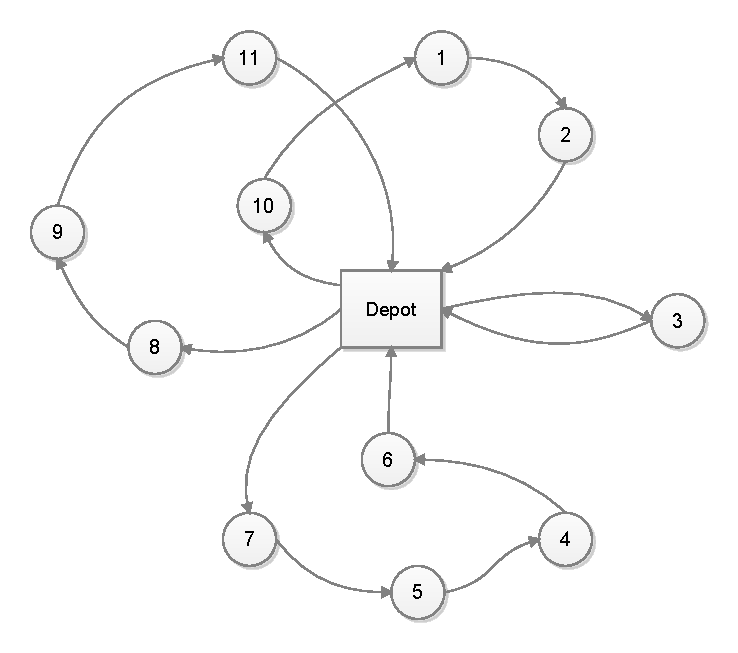
\includegraphics{images/vrpbasic.pdf}
    \caption{An example of a VRP solution}
    \label{fig:simplenetwork}
  \end{center}
\end{figure}

\section{Classical vehicle routing problem}



The basic VRP can be defined with an graph $G = (V, A)$ where $V = \{v_1, v_2, v_3\dots\}$ represents the vertices, ie. the depot and targets for the visitations and $A = \{(v_i, v_j): i \neq j \}$ represents the arcs between the vertices. The vertex $v_0$ typically represents the depot. For every arc, there is a non-negative travel cost $C=(c_{ij})$. In this context, it is used to represent the traveling time between vertices. If the travel cost is symmetric between all pairs of vertices, an undirected graph $G = (V, E)$ can be used instead, where $E=\{(i, j) : i, j \in V, i < j\}$. In all cases, the end result is an all-to-all network. \cite{laporte2007you} 

The main idea in the network is that every node (i.e. vertex) has a connecting edge to every other node. Even if in real life there would be overlapping in the routes as one road probably leads to more than just one node, for the sake of the problem the edges are considered unique, as can be seen in Figure~\ref{fig:reallifenetwork}. In other words, even though the road map of a country does not consist of an all-to-all type network topology, the mathematical model used for this problem uses one. 

\begin{figure}[h]
  \begin{center}
    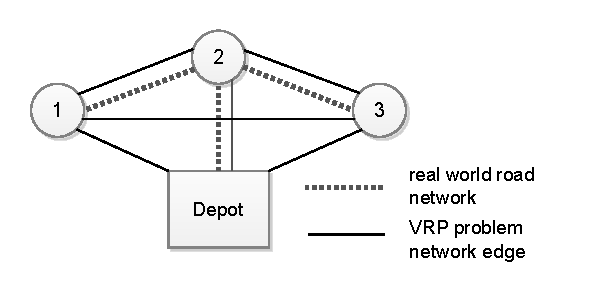
\includegraphics{images/simplenetwork.pdf}
    \caption{Real life network and the mathematical network}
    \label{fig:reallifenetwork}
  \end{center}
\end{figure}

The first vertex in $V$ represents the depot, where all the vehicles start from and where they must end their trips. $m$ identical vehicles have a capacity denoted by $Q$ which symbolises the resources available for each trip. In the classic VRP, $m$ is logically equivalent to the number of trips needed to visit every customer. With time windows this no longer holds true. Every customer vertex $i \in V\setminus\{v_0\}$ has a demand $q_i \leq Q$ associated with it. This symbolises the various resources, including time, required at the target. \cite{laporte2007you}

Vehicle routing problem is NP-hard as it is a superset of the traveling salesman problem. In traveling salesman problem, the number of vehicles is $m = 1$, there is no upper limit on the costs of a route and the capacity of the vehicle is greater than the combined requirement of all the nodes in the network ($Q = \infty$). \cite{laporte2007you} The classic VRP is sometimes called the capacitated vehicle routing problem (CVRP). \cite{hassanzadeh2009location}

Let $x_{ij}$ denote the number of trips made over the edge $[i, j]$ in a solution. The total cost that should be minimised is then:

\begin{equation}
\label{eq:baseformula1}
\displaystyle \sum_{[i,j] \in E} c_{ij}x_{ij}.
\end{equation}

\noindent
The following conditions must hold true:

\begin{equation}
\label{eq:baseformula2}
\displaystyle \sum_{j \in V \setminus\{0\}} x_{0j} = 2m,
\end{equation}

\noindent
meaning that given $m$ routes, the edges between the depot and other vertices are used exactly $2m$ times, as seen in Figure~\ref{fig:basecond1}. \cite{laporte2007you}
\begin{figure}[h]
  \begin{center}
    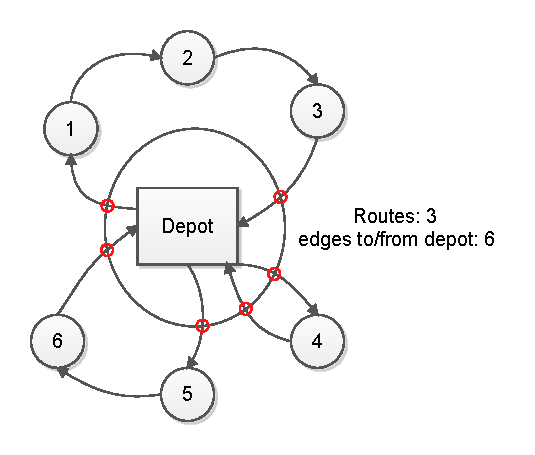
\includegraphics{images/basecond1.pdf}
    \caption{Routes to and from the depot}
    \label{fig:basecond1}
  \end{center}
\end{figure}

\begin{equation}
\begin{aligned}
\label{eq:baseformula3}
\displaystyle\sum_{i < k} x_{ik} + \displaystyle\sum_{j > k} x_{kj} = 2 && (k \in V \setminus\{0\}),
\end{aligned}
\end{equation}

\noindent
meaning that every vertex that is not the depot has two connecting edges that are used in the solution. In other words, every non-depot vertex is visited exactly once. \cite{laporte2007you}

\medskip
\noindent
If $b(S)$ represents the minimum number of vehicles required to satisfy the needs of the customers of $S$, the constraint

\begin{equation}
\begin{aligned}
\label{eq:baseformula4}
\displaystyle\sum_{\substack{i \in S, j \notin S \\ 
\text{ or } i \notin S, j \in S}} x_{ij} \geq 2b(S) && (S \subset V \setminus\{0\}).
\end{aligned}
\end{equation}

\noindent
means the number of edges travelled between the vertices in the network contained in S and the vertices of the rest of the network has to be at least 2 times the minimum number of vehicles required to satisfy the needs of the customers of $S$. \cite{laporte2007you}



\begin{equation}
\begin{aligned}
\label{eq:baseformula5}
x_{i,j} = 0 \text{ or } 1 && (i, j \in V\setminus\{0\})
\end{aligned}
\end{equation}

\noindent
and

\begin{equation}
\begin{aligned}
\label{eq:baseformula6}
x_{0,j} = 0, 1 \text{ or } 2 && (j \in V\setminus\{0\})
\end{aligned}
\end{equation}

\noindent
mean that every edge whose other end is the depot is travelled at most two times, while the rest of the edges are traveled once at most. \cite{laporte2007you}







\section{Variations of the vehicle routing problem}

The real life needs of route planning are rarely satisfied with the basic vehicle routing problem. There are typically additional constraints and an increased complexity that require expanding the problem statement. The vehicles used are probably not identical in terms of capacity and cost. The number of depots might also be greater than 1 and each target has to be allocated to one of them. \cite{salhi2014multi} In addition, there might be specific time windows during which the targets have to be visited \cite{ghoseiri2010multi}. 

All of these additional features can be combined into a multitude of variations of the VRP. As all the variations add to the complexity of the VRP, they too are NP-hard. The variations listed here represent the most common types of VRP, but in addition, there are more specific types still available, such as one where only certain types of vehicles may visit certain targets. \cite{montoya2015literature} 


\subsection{Multi-depot Vehicle routing problem}

Multi-depot Vehicle routing problem (MDVRP) is a variation of VRP where there are additional depots which can be utilised as the start and end points of routes as can be seen in Figure~\ref{fig:multidepot}. A vehicle must start and end the route at the same depot. While at first it might seem that MDVRP can be just split into multiple single depot VRPs by assigning each target to the nearest depot, this leads to suboptimal solutions. \cite{salhi2014multi}

\begin{figure}[h]
  \begin{center}
    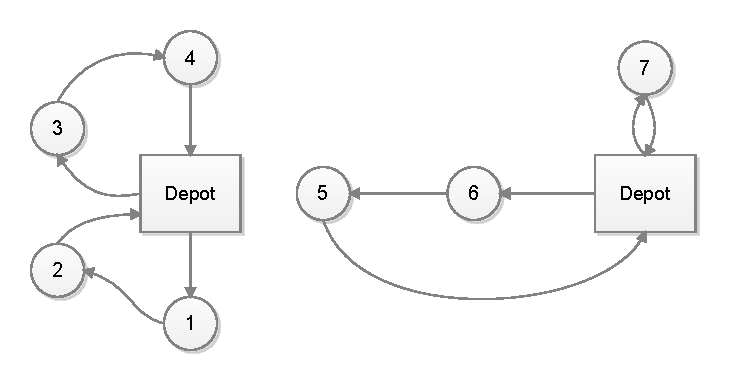
\includegraphics{images/multidepot.pdf}
    \caption{A VRP with two depots}
    \label{fig:multidepot}
  \end{center}
\end{figure}

\subsection{Heterogenous fleet vehicle routing problem}

In real world scenarios, it is uncommon that all the vehicles in a fleet are identical. A typical variation of the VRP called heterogenous fleet vehicle routing problem (HVRP) one where the vehicles are not assumed to be identical. There is a fixed cost associated with each vehicle type and a variable cost per distance unit. Vehicle types also have unique capacities which play an important role in route generation. \cite{gendreau1999tabu}


\subsection{Vehicle routing problem with time windows}

Time windows and other scheduling constraints are common in real world and thus including them in VRP is crucial in order to get results that are applicable in common business cases. These can include postal, food or cargo delivery and service visits where it is common that the customer wants the delivery to occur during a specific time. \cite{cordeau2000vrp}

To define vehicle routing problem with time windows (VRPTW), let $s_i$ denote the time that a vehicle has to spend at a target $i$ and $b_i$ denote the time at which the delivery of the service or goods begins. The earliest time the target accepts the start of the delivery is $e_i$ and the latest is $l_i$. If a vehicle arrives too early at $j$, it will have to wait so that the earliest time it can deliver the goods or services is $b_i = \max\{e_j, b_i + s_i + t_{ij}\}$. Here $t_{ij}$ represents the time required to travel between $i$ and $j$. \cite{solomon1987algorithms}


\subsection{Vehicle routing problem with pickup and delivery}

Vehicle routing problem with pickup and delivery (VRPPD) defines a VRP where a set of transportation requests must be satisfied. The requests all have a pickup point and a delivery point where the goods or passenger has to be brought. In case of passengers, a common application in real life can be found in taxi service. A courier service would be an example of a scenario where goods need to be transported from one point to another. Due to the nature of the applications for VRPPD, it is usually combined with VRPTW. The standard VRP is a VRPPD where the pickup point is always the depot and the delivery points are spread out elsewhere or vice versa. \cite{desaulniers2000vrp}


\subsection{Periodic vehicle routing problem}

While the classic VRP assumes a single time period, a single day for example, during which a deliveries have to be made, periodic vehicle routing problem (PVRP) defines a case with repeating time windows. Customers may need to be visited once or multiple times, and they may require the visit to occur on a specific weekday. \cite{blakeley2003optimizing} Common applications for the PVRP include waste collection, vending machine replenishment and cleaning service. PVRP is commonly combined with VRPTW as it is likely that in addition to wanting the visit to take place on a specific day, the customers also have requirements regarding the time of the visit. \cite{yu2011ant}


\subsection{Location routing problem}

In location routing problem (LRP), the location of the depots has to be determined before creating the routes. The factors that have to be taken into account are the one time and running costs of the depots and the traveling costs that are based on the locations of the depots. The main objective is to position the depots as close to the customers as possible. In practice, the maximum size of the depot is also limited. A large depot in a city centrum might incur too large costs in order to be feasible. Once the locations of the depots has been decided, the problem turns into a multi-depot vehicle routing problem, though naturally the positions can be altered at any point during the solving. \cite{tuzun1999two}


\subsection{Green vehicle routing problem}

Due to the apparent need to cut down $CO^2$ emissions and the fact that the vast majority of vehicles, especially heavy transport, run on fossil fuels, there is an increasing motivation to pay more attention to the environmental aspects of transportation. Green vehicle routing problem (GVRP, also known as emissions vehicle routing problem) aims to minimise emissions and helps routing for vehicles that may require special fueling stations. \cite{erdougan2012green}



\section{VRP solutions}

In this section I present some common algorithms to produce solutions to various VRPs. Because there are so many different types of VRP and each having its own set of solving methods, only the most common ones are listed here. In chapter~\ref{chapter:implementation} I will more closely analyse which additional VRP features are required in the business case of this thesis. Then I will analyse which of these solutions methods will be most suitable to produce usable solutions.

There are three main categories of VRP solving algorithms. The first category consists of algorithms that produce exact solutions. Due to the complexity of VRP, exact algorithms can only handle networks with up to about 100 nodes. This has resulted in the bulk of the research focusing on the two main types of heuristics: Classical heuristics and metaheuristics. \cite{laporte2007you}  

Classical heuristics produce good results in reasonable computing time and cover the bulk of most modern heuristics in use. They are also easily suited for real world constraints and requirements. In metaheuristics, the most promising solution space is further explored. They employ advanced neighbourhood search patterns, memory structures and commonly use recombinations of solutions to find better ones. The downside is increased complexity and computational requirements, but they typically produce higher quality solutions. \cite{laporte2000classical}

For notation, we will use (0, $i$, $j$, $k$, 0) to denote a route that starts at depot 0 and goes to targets $i$, $j$ and $k$ before returning to the depot. In case of multiple depots, they will be denoted with other indexes, e.g. (1, $l$, $m$, 1).



\subsection{Savings algorithm}

The savings algorithm is one of the most basic algorithms for VRP. It assumes that the number of vehicles is a decision variable. Figure~\ref{fig:savings1} shows an example of how the savings algorithm progresses.

\begin{figure}[h]
  \begin{center}
    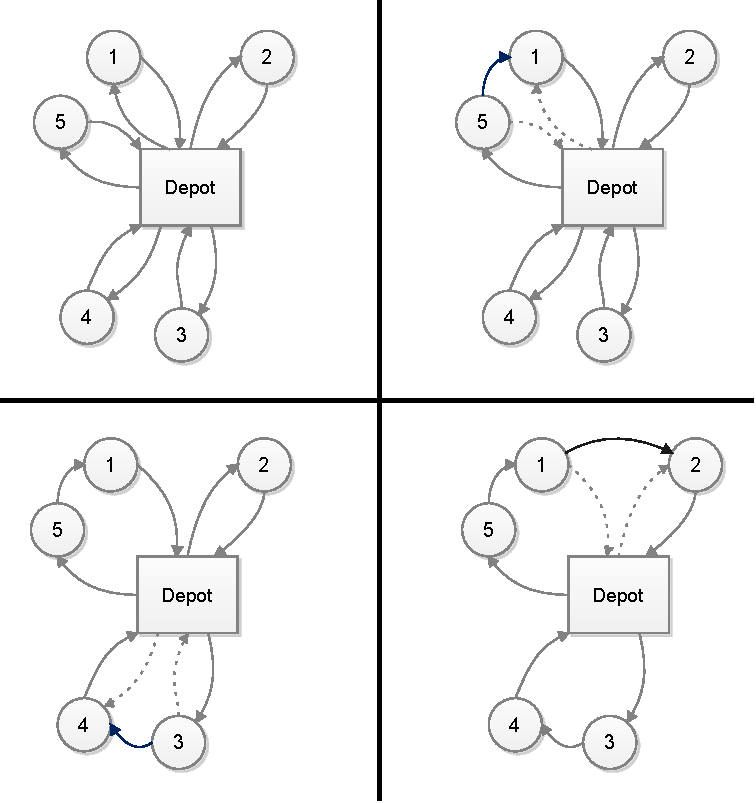
\includegraphics{images/Savings1.pdf}
    \caption{An example of savings algorithm progression where car capacity is 3 and demand per node is 1}
    \label{fig:savings1}
  \end{center}
\end{figure}

\bigskip
\noindent
Create one vehicle route per node so that the route just goes to the target and comes back to the depot. This will result in $n$ vehicle routes (0, $i$, 0) for $i = 1, \ldots, n$. \cite{reimann2004d}

\medskip
\noindent
\textbf{Step 1:} Calculate \textit{savings}: $s_{ij} = c_{i0} + c_{0j} - c_{ij} \text{ for } i, j = 1, \ldots, n \text{ and } i \neq j$. Sort the savings in descending order. \cite{reimann2004d} At the top of the savings list are then pairs of targets who are farthest away from the depot and closest to each other. Essentially this gives us the clue that they should probably be merged into the same route. There are two common ways to use the savings list.


\medskip
\noindent
\textbf{Step 2 (best savings first):} Starting from the top of the savings list, see if the routes can be merged so that the saving $s_{ij}$ causes the removal of $(0, j)$ and $(i, 0)$ and the addition of $(i, j)$. \cite{reimann2004d} This means that no routes will be cut in half during the algorithm, but that routes are merged from end to end, excluding the depot.

\medskip
\noindent
\textbf{Step 2 (route first):} For each route $(0, i, \ldots, j, 0)$, find the first saving $s_{ki}$ or $s_{jl}$ that allows merging of another route that either ends with $(k, 0)$ or starts with $(0, l)$. Merge these two routes and continue the operation until no more feasible merges exist. Then move on to the next route and start all over again. \cite{laporte2000classical}

 



\subsection{Sweep algorithm}			

Popularised by Gillet and Miller in 1974, the sweep algorithm is usable on data sets where the coordinates of the targets are known. It is based on calculating the polar coordinates between the depot and the targets so that one arbitarily chosen target represents the zero angle. The targets are then sorted according to the polar angle. The sorted targets are added in order to the new route until the cost or capacity limit of a single route has been reached and no more new targets can be inserted. Then a new route is created and the algorithm is repeated until all targets have been assigned to a route. \cite{gillett1974heuristic}

The found routes are then optimised with any traveling salesman solver. Since the routes are supposedly relatively small at this point, solving the individual TSPs should be a lightweight operation. Once each route has been initially created and optimised, the algorithm then tries to swap neighbour routes' targets according to their distance from the depot and the angle to the next route. If the swap improves the solution, the target is moved to the other route. After no more improvements can be found through swapping, the algorithm finishes. \cite{gillett1974heuristic} Figure~\ref{fig:sweep1} shows an example of how the sweep algorithm works in practice. 

The downside to this heuristic is that it doesn't take the road network into account during the sweep. It assumes that the geometrical distance is the most important piece of criteria. To counter this, it is typical to run the algorithm so that all targets get picked to be as the beginning point of the sweep. \cite{reimann2004d} 


\begin{figure}[h]
  \begin{center}
    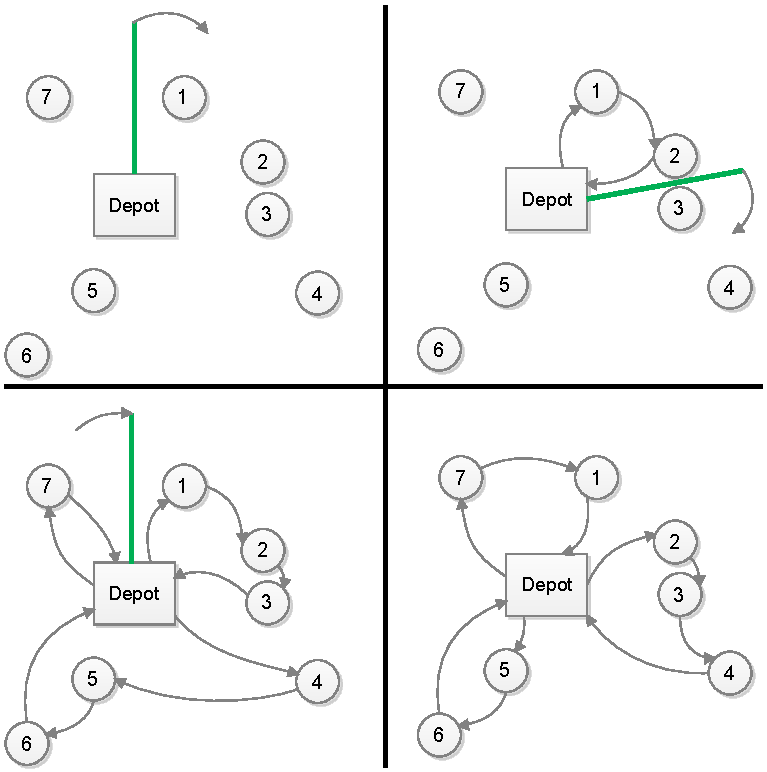
\includegraphics{images/Sweep1.pdf}
    \caption{An example of sweep algorithm progression where car capacity is 3 and demand per node is 1. In the final iteration some routes swap nodes to produce more optimal solution.}
    \label{fig:sweep1}
  \end{center}
\end{figure}

\subsection{Petal algorithm}

The petal algorithm resembles the sweep algorithm, as all the targets are first sorted according to their polar angle from the depot and an arbitarily chosen point. A set $S$ of possible routes called petals is then generated and optimised using TSP as above. The problem is then formulated as follows:


\bigskip
\noindent
Minimise

\begin{equation}
\label{eq:petal1}
\displaystyle\sum_{\substack{k \in S}} d_kx_k
\end{equation}


\noindent
where $S$ is the set of all routes in the set, $x_k = 1$ if and only if route k is part of the solution and $d_k$ represents the cost of the whole route $k$. Apply the following conditions:

\begin{equation}
\begin{aligned}
\label{eq:petal2}
\displaystyle\sum_{\substack{k \in S}} a_{ik}x_k = 1 && i = 1, \ldots, n
\end{aligned}
\end{equation}

\noindent
and

\begin{equation}
\begin{aligned}
\label{eq:petal3}
x_{k} = 0 \text{ or } 1 && k \in S
\end{aligned}
\end{equation}

where $a_{ik}$ is 1 only if the vertex $i$ is in the route $k$. \cite{laporte2000classical} The conditions state that every vertex belongs to exactly one route. The Sweep and petal algorithms are classic examples of ``cluster-fist route-second'' types of algorithms, where first the targets are grouped and then for those groups, the optimal routes are discovered. 

\subsection{2-petal algorithm}

\subsection{Tabu search}

\subsection{Greedy Randomized Adaptive Search Procedure (GRASP)}

\subsection {Ruin and Recreate}

Developed by Schrimpf et al., the ruin and recreate algorithm is based on the concept of having a solution of varying quality as the base, after which all trips to a set of nodes are removed (``ruined''). The set can be picked randomly, from a radial area, or by some other rule. The intermediate result is the same solution as in the beginning, with some nodes not being serviced. The routes are then re-created so that every ruined node gets inserted into a route where it creates the least amount of additional time requirement so that no constraints (capacity, time, etc.) are broken. If it is impossible to insert a ruined node to a route without breaking constraints, a new route will be created. Once all the ruined nodes have been readded to routes, the algorithm can be repeated. \cite{schrimpf2000record} 

Shrimpf et al. state that there are probably better and more elaborate algorithms for the recreation procedure, but that even with their simple scheme, very good results can be achieved. Likewise, there are numerous strategies to choose from for the ruin part of the algorithm. Also, choosing which solution to continue from after iterations affects results. One way is to always use the best results gotten so far, but it may also pay off to try to continue from a slightly worse solution. A big benefit of the algorithm is that it allows easy applying of custom constraints. \cite{schrimpf2000record} 

This algorithm is used in the library I picked to use for the VRP program. In addition it employs features presented by Pisinger and Ropke\cite{pisinger2007general}.

TODO: add graph demonstration, expand on the various strategies in the phases of the algorithm.

\subsection{Genetic algorithm}

\subsection{Ant colony}

\subsection{Bee colony}

\chapter{Methods}
\label{chapter:methods}

The basic problem can be divided into two parts. First is abstracting the business data into numbers and the second is applying the found numbers into the chosen vehicle routing problem algorithm. The business data includes locations of the job targets and the depots and the man-hour and equipment requirements of the jobs.  

\section{Abstracting the problem field into numerical data}

Raw data from the client company's database is unusable by itself. It needs to be transformed into abstract numbers that can be used as parameters for the routing heuristic. The goal is to minimise the number of variables to prevent the actual algorithm from becoming overly complex while still ensuring that all available information is taken into account when generating the solution. 

\subsection{Generating the distance matrix}

One problem in the project is transforming the location data, mainly addresses, into form that can be more readily be used programmatically. The goal is to produce a matrix that lists the travelling time units between all the targets, including the depot. Because of the large number of targets, it is reasonable to optimise this step by grouping nearby targets together. Grouping should be done so that the traveling time between them is negligible and thus not much information is lost by the operation. The end result is that as far as the algorithm is concerned, the grouped targets occupy the same address.

Because the addresses of the customers are inputted by hand into the database of the client company, not all of them are valid. Some have typos, while others may have the wrong municipality due misinformation or the frequent merges in the country. To mitigate this problem, the user can re-enter the address in case the routing service does not recognise it. Another option is to group the job with already existing jobs.

Choosing a suitable routing service is an important decision to be made in the early development. Generating the many-to-many traveling time matrix required in this project quickly cause an increase in the number of queries required. The licence fees which are typically based on the number of queries made within a time period must be kept reasonable.

Naturally the routing service has to support Finland's addresses and roadmap. Another important requirement is that it can estimate the traveling time between targets, because distance by itself is not very descriptive due to varying speed limits on different roads. Traffic congestion will probably be impossible to take into account because the driving will take place weeks into the future and also because the exact time and date are not known at the time of the query. 

One possible way to take congestion into account would be to redo the queries after an initial solution has been generated if the routing service can predict traffic based on previous dates' data and then adjust the solution if needed. However, the potential benefits would be limited at best and would not justify the increased complexity.


\subsection{Calculating job costs}

NOTE: number of technicians might always be one. This needs checking. Overall this is a very crude sketch of the subsection. 

To prevent the algorithm from becoming overly complex, the time and resource requirements of a single job should be simplified as much as possible. The input:

\begin{itemize}
\item Types and number of tasks involved in the job
\item Installation items and equipment required.
\item Minimum number of technicians required.
\item The assigned technician's performance if a specific technician is required for the job.   
\end{itemize}

The end result should be the following parameters per job target:

\begin{itemize}
\item Vehicle capacity requirements of the installation items and other equipment.
\item Minimum number of technicians required at the job.
\item Total time requirement for the technicians assuming that the number of technicians is the minimum number.  
\end{itemize}

Each task type has a unique time cost associated with it which is then adjusted with various factors. Different house types, floors and other environmental conditions affect on how much time is required per task. The type and size of item to be installed into the house also plays a role. 

The number of technicians required at a job target is a hard parameter, in that one technician working twice as long will not be able to complete the task. If even a single task at the target requires more than one technician, the whole job will be considered a two-person job. 

Two people do not perform twice as fast as a single person and different tasks at a job benefit different amounts from an increased workforce. Therefore the benefit from additional technicians should be estimated per type of task. 



% TODO: generate a generic way to include new tasks, resources, house types and how they affect the total job requirements.
% TODO: how the algorithm parameters fit into this. 
 
\chapter{Implementation}
\label{chapter:implementation}

My experiences during the whole ordeal

\section{Technical decisions}

Picking libraries, choosing languages, determining algorithms, yeah!


\subsection{Choosing the libraries to use}

The important criteria for choosing the libraries to use are performance, solution quality and suitability to the parameters specific to this project. Ease of use and the quality of documentation are also signifcant factors.

Since there are so many different variations of the VRP, finding one which satisfies the requirements of the business context of this project will be challenging, and may require adapting the parameters to make them compatible with the library API. If that is not possible, writing an algorithm of my own will be necessary.


\subsection{Language requirements}

The most important aspect of choosing which language to use depends on the routing algorithm libraries available for the language. 

Because the algorithm is CPU-intensive, the more low-level languages take precedence over the potentially slower high-level languages. This is not a deciding factor, however, as many of the high-level languages are still sufficiently fast enough for this purpose. Likewise, even if a program written in pure C, for example, might perform better, the increased development time and reduced maintainability are more significant significant issues than a slightly reduced performance of a Java program.

Due to the performance-centric nature of the algorithm, it is important that the language chosen can be profiled to see which parts of the algorithm are the most resource-intensive. Though most modern languages fulfill this requirement, it is worthy of mentioning.


\subsection{Langugage and library decision}

What did I choose?

\section{Development of the program}

\subsection{Structure of the program}

To ensure future maintainability, the program should be modular, so if some part of the program needs to changed, the operation would be as easy as possible. The modules of the program would be as follows:

\begin{enumerate}  
\item Routing module, transforming address data into a traveling cost matrix.
\item Job resource calculator, abstracting the job resource and man-hour requirements into numbers.
\item The algorithm module, using the traveling cost matrix and job requirements to produce route data.
\item Results visualiser, displaying the results data in a more human-readable form.
\item Results storing module, converting the results into data suitable to be stored in the client company's database. 
\end{enumerate}

 

\chapter{Evaluation}
\label{chapter:evaluation}

How my solution worked out. How comparable it is to existing models? What are the time requirements with the data given? How optimal are the solutions? Is the software future-proof?


\section{Customer's perspective}

If I ended up trying many different algorithms or if I wrote my own, how did they compare?



\section{Future development}

This and this went wrong. This caused trouble.


\section{Retrospective}

What I would've done differently with the knowledge I have now.
 
\chapter{Conclusions}
\label{chapter:discussion}

There are so many various trades whose operation or parts of it can be abstracted to a VRP that there is much room for improvement in terms of automation in our society. It is no wonder that so much research has been done on the subject. Any sufficiently large company will probably benefit from applying it to various processes unless their everyday problems have absolutely nothing to do with VRPs.

The basic requirement for benefitting from this kind of work planning is having some sort of formalised database to which customer information is being stored. Then it is possible to transform that data and use it to solve the VRP associated with the business at hand. Naturally there are many trades which do not have anything in common with VRPs, but many aspects around the basic necessities of modern human life heavily involve concepts related to VRPs. Delivery of food and other goods from producers to intermediate storages and furthermore to markets are a prime example, and if grocery deliveries straight to the doorstep becomes more common, there will be yet another common application for VRPs.  

Even if in this specific case there was not much of a benefit in using an advanced solver, there was no downside to it either. The main benefit in this case was simply the automation process and providing a framework upon which future development can be based. A job which once required human labour has now been partly replaced by a machine. Furthermore, if the client company takes this work planning automation further, it is entirely possible to reach a point where only on specific exceptional circumstances does the process require any human interaction at all. 

Based on my experiences with this project, I am certain that automating this kind of work planning would bring great benefit to a lot of companies. Though businesses are different and each has its own unique set of requirements, versatile libraries such as Jsprit could probably be used for their purposes. The biggest work would be adapting the business model into an algorithmic format. A general solution would work only in select cases where the business model of the companies is automatically translated into a certain variation of a VRP. Otherwise customisation is needed, meaning that for small scale operations, automatisation might not be cost effective. 

The open source library Jsprit continues the good trend of increasing number of free tools being available to the general public. It is a good example how free software can be used to make human societies more efficient. This will eventually and ultimately lead to humankind having more free time as workforce is replaced by machines. Assuming that this redistribution of work is taken into account on a political level (a huge assumption that does not hold true so far, admittedly), humankind can only benefit from this development.



 
\chapter{Conclusions}
\label{chapter:conclusions}

A nice concise summary of what I have done and how well that has worked out.


% Load the bibliographic references
% ------------------------------------------------------------------
% You can use several .bib files:
% \bibliography{thesis_sources,ietf_sources}
\bibliography{sources}


% Appendices go here
% ------------------------------------------------------------------
% If you do not have appendices, comment out the following lines
% \appendix
% \chapter{First appendix}
\label{chapter:first-appendix}

Nothing here so far.

% End of document!
% ------------------------------------------------------------------
% The LastPage package automatically places a label on the last page.
% That works better than placing a label here manually, because the
% label might not go to the actual last page, if LaTeX needs to place
% floats (that is, figures, tables, and such) to the end of the 
% document.
\end{document}
